% HEADER
\documentclass[class=article, crop=false]{standalone}
\usepackage{00_Preamble/frr_preamble}

% Packages
\usepackage{titlesec}
\usepackage{hyperref}
\usepackage{float}
\usepackage{graphics}
\usepackage{placeins}
\usepackage{adjustbox}
\usepackage{array}


\renewcommand{\arraystretch}{1.4}
% END HEADER

\begin{document}
	\subsection{Preliminary Design}
	\label{subsec:preliminary_design}
	Each system on the robot went through multiple design iterations during the preliminary design process. Significant background research was conducted into the Mars environment, potential excavation systems, drivetrain, and path planning and SLAM implementations. Trade studies were combined with testing to determine the best and most realistic rover design.
	\subsubsection{Drive System}
	Significant research was done on the drive systems of other RMC teams from previous years. Many robots encountered wheel slippage and struggled to maneuver out of steep ditches. The primary goal of robot drive system was to provide traction in BP-1 and avoid obstacles and ditches in the terrain. 
	
Two potential drive mechanisms were considered: a 4-wheel direct drive and tank tread drive. A trade study for the drive systems considered is shown in Table \ref{table:drive_trade_study}. Both systems present unique fabrication challenges. The tank tread drive has more moving parts than the wheels, but the wheels would require significantly more custom manufacturing since few off-the-shelf wheels are available that meet the system requirements. As a result of the increased number of moving parts, the tank tread drive is also less power-efficient than the four wheel direct drive.  Both systems present unique fabrication challenges. The tank tread drive has more moving parts than the wheels, but the wheels would require significantly more custom manufacturing since few off-the-shelf wheels are available that meet the system requirements. As a result of the increased number of moving parts, the tank tread drive is also less power-efficient than the four wheel direct drive.  The ability to independently drive each wheel improves maneuverability and stability when climbing obstacles. However, this comes at the cost of increased control system complexity over the tank tread drive.   The 4-wheel direct drive also provides redundancy as the system is fail-operational in the case a of single drive motor failure. Due to the simple design implementation and the increased maneuverability, the four-wheel skid-steer system was selected.

\FloatBarrier
	\begin{table}[h]
	\footnotesize
	\centering
	\begin{tabular}{ | p{8em} | m{4em} | m{6em} | m{3em} | m{8em} | m{3em} | }
 	\hline
 		\rowcolor[gray]{0.8}
 		\textbf{Factor} &\textbf{Weight} &\textbf{Tank Tread Drive} &\textbf{Score} &\textbf{4-Wheel Direct Drive} &\textbf{Score}  \\ 
 		\hline
		Fabrication                       &  \multicolumn{1}{c|}{0.7}  &  \multicolumn{1}{c|}{8}    &  \multicolumn{1}{c|}{5.6}  &  \multicolumn{1}{c|}{4}    &  \multicolumn{1}{c|}{2.8}   \\ 
 		\hline
 		Obstacle \mbox{Avoidance}         &  \multicolumn{1}{c|}{0.9}  &  \multicolumn{1}{c|}{7}    &  \multicolumn{1}{c|}{6.3}  &  \multicolumn{1}{c|}{9}    &  \multicolumn{1}{c|}{8.1}   \\ 
 		\hline
 		\mbox{Control System} Complexity  &  \multicolumn{1}{c|}{0.6}  &  \multicolumn{1}{c|}{9}    &  \multicolumn{1}{c|}{5.4}  &  \multicolumn{1}{c|}{6}    &  \multicolumn{1}{c|}{3.6}   \\
 		\hline
 		Power \mbox{Efficiency}           &  \multicolumn{1}{c|}{0.4}  &  \multicolumn{1}{c|}{5}    &  \multicolumn{1}{c|}{2}    &  \multicolumn{1}{c|}{9}    &  \multicolumn{1}{c|}{3.6}   \\ 
 		\hline
 		Obstacle \mbox{Traversal}         &  \multicolumn{1}{c|}{0.7}  &  \multicolumn{1}{c|}{8}    &  \multicolumn{1}{c|}{5.6}  &  \multicolumn{1}{c|}{7}    &  \multicolumn{1}{c|}{4.9}   \\
 		\hline
 		\mbox{Reliability and} Simplicity &  \multicolumn{1}{c|}{0.6}  &  \multicolumn{1}{c|}{4}    &  \multicolumn{1}{c|}{2.4}  &  \multicolumn{1}{c|}{9}    &  \multicolumn{1}{c|}{5.4}   \\
 		\hline
 		\rowcolor[gray]{0.9}
 		\textbf{Total}                    &       &       &\multicolumn{1}{c|}{\textbf{27.3}}&       &\multicolumn{1}{c|}{\textbf{28.4}}\\
 		\hline
	\end{tabular}
	\caption{Trade Study Matrix for Drive System }
		\label{table:drive_trade_study}
	\end{table}
	\FloatBarrier
	
	\subsubsection{Wheels}
	The wheels were designed to find a compromise between traction, obstacle-traversal ability, weight, and build complexity. The preliminary wheel design can be seen in Figure \ref{fig:cad-wheel-prelim}. The wheels have a 30 cm diameter to be able to climb over smaller obstacles. Based on research into rover wheel design, the team determined that grousers were required to provide traction in the loose BP-1. 12 grousers were chosen to be a good compromise between traction and a smooth ride to vibration and sensor noise. The red spacers are 3D printed to fasten the grousers, wheel sides, and rim together. 6061-T6 aluminum was selected due to its low weight, relatively high strength, and machinability.
	
	\FloatBarrier
		\begin{figure}[h]
			\centering
			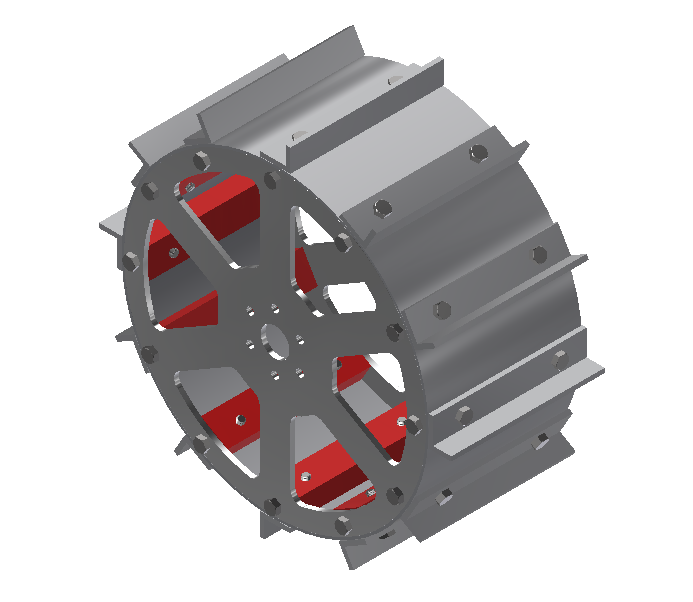
\includegraphics[width=0.4\linewidth]{09_Figures/wheel-cad-preliminary.jpg}
			\caption{CAD model of preliminary wheel design.}
			\label{fig:cad-wheel-prelim}
		\end{figure}
		\FloatBarrier

	\subsubsection{Excavation}
	The driving requirement for the excavation system was to dig through the 30 cm of BP-1 and collect the gravel underneath. The primary design considerations for the digging mechanism were reliability, dust tolerance, complexity, and weight. 
Research was performed on existing digging mechanisms in the mining industry. Refer to Figure X for a trade study of the designs. The backhoe and bucket wheel excavator were eliminated from the solution space as they are primarily effective for surface mining.  The bucket wheel excavator is capable of removing a large amount of material, but it does not fit within the size constraints of the robot., but its large size would make it hard to fit within the size constraints. 

The chain trencher would be able to excavate significantly more gravel than an auger. However, the power requirements are immense, which is why chain trenchers are always gasoline-powered. After consulting with engineers at Ditch Witch, it was determined that a chain trencher of the correct scale for the RMC would require at least 4 HP to run. This power requirement was not worth the increased gravel collection. 
The auger was the team’s chosen digging mechanism. It provided a compromise between weight, power consumption, and the mass of gravel collected. The biggest concern was whether the auger would be able to excavate large gravel particles, as augers are generally used for liquids and fine particulate. The team ran experiments to test the auger’s ability to dig through sand and gravel with a tube covering that funnels up gravel. The tube covering was successful in allowing material to be conveyed up the blade. Refer to Appendix A for data from the experiment.

\FloatBarrier
	\begin{table}[h]
	\scriptsize
	\centering
	\begin{tabular}{ | r | c | c | c | c | c | c | c | c | c | c |}
 	\hline
 		\rowcolor[gray]{0.8}
 		\textbf{.} &\textbf{Cost} &\textbf{Fabrication} &\textbf{Power} &\makecell{\textbf{Operative} \\ \textbf{Complexity}} &\textbf{Robustness} &\makecell{\textbf{Scoring} \\ \textbf{Potential}} &\textbf{Mass} & \makecell{\textbf{Ease of} \\ \textbf{Integration}} &\textbf{Size} &  \\ 
 		\hline
		\makecell{\textbf{Decision} \\ \textbf{Weight:}}& \textbf{0.1} &\textbf{0.15} &\textbf{0.1} &\textbf{0.05} &\textbf{0.05} &\textbf{0.2} &
		\textbf{0.1} &\textbf{0.1}  &\textbf{0.15} &\makecell{\textbf{\underline{Weighted}} \\ \textbf{\underline{Score}}}  \\ 
 		\hline\hline
 		\makecell{\textbf{Auger and} \\ \textbf{Tube}}    & 8 & 8 & 7 & 8 & 6 & 3 & 6 & 5 & 7 & \textbf{6.15} \\ 
 		\hline
 		\makecell{\textbf{Chain} \\ \textbf{Trencher}}    & 6 & 8 & 1 & 9 & 7 & 10 & 2 & 3 & 2 & \textbf{5.5} \\
 		\hline
 		\makecell{\textbf{Bucket} \\ \textbf{Excavator}}  & 6 & 5 & 4 & 7 & 3 & 1 & 7 & 10 & 6 & \textbf{4.05} \\
 		\hline
 		\makecell{\textbf{Plow and} \\ \textbf{Back-hoe}} & 5 & 5 & 4 & 5 & 2 & 2 & 3 & 2 & 2 & \textbf{3.2} \\
 		\hline
 		\makecell{\textbf{Circular} \\ \textbf{Excavator}}& 5 & 2 & 6 & 8 & 3 & 6 & 2 & 7 & 1 & \textbf{4.2} \\ 
 		\hline
	\end{tabular}
	\caption{Trade Study Matrix for Digging Mechanism}
		\label{table:dig-trade-study}
	\end{table}
	\FloatBarrier
	
	
	
	
	


	
\end{document}
